% importa variabili globali
% definizione variabili globali
\def\GRUPPO {\textit{DazzleWorks}}

\def\PROGETTO {\textbf{Premi}}

\def\COMMITTENTE {Prof. Vardanega Tullio, \\ & Dr. Cardin Riccardo}

\def\EMAIL {dazzleworksgroup@gmail.com}

\def\LOGO {../../template/img/logo.png}

\def\INTESTAZIONE {../../template/img/intestazione.png}
\def\PIEDIPAGINA {../../template/img/piedipagina.png}

\def\G {{\small $_G$}}



% definizione variabili locali
\def\DOCUMENTO{Norme di Progetto}
\def\VERSIONE{3.0.0}

\def\DESCRIZIONE{Documento contenente l'insieme di norme stabilite dal gruppo \GRUPPO per la realizzazione del progetto didattico \PROGETTO.}

\def\REDATTORE {Burlin Valerio}
\def\VERIFICATORE {Ros Fabio}
\def\RESPONSABILE {Suierica Bogdan}

\def\USO {Interno}

\def\DISTRIBUZIONE {\GRUPPO{}\\ & \COMMITTENTE{}\\}

\def\DESCRIZIONE {Documento contenente l'insieme di norme stabilite dal gruppo \GRUPPO\ per la realizzazione di \PROGETTO.}


% abilita (true) / disabilita (false) indice, lista tabelle, lista figure
\def\INDICE	{true}
\def\TABELLE {false}
\def\FIGURE {true}


% importa struttura
\documentclass[a4paper]{article}

% ----- definizioni -----
\def\TITLE		{\mbox{\GRUPPO}}
\def\SUBTITLE	{\SIGLA, \PROGETTO}


% ----- nuovi comandi -----
% fornisce il caption per riferirsi ad una particolare sezione
\newcommand{\numref}[1]{\textsf{\textsl{``\nameref{#1}'' (\ref{#1})}}}


% ----- package -----
\usepackage[T1]{fontenc}   % codifica dei font in uscita
\usepackage[utf8x]{inputenc}   % lettere accentate da tastiera
\usepackage[italian]{babel}   % lingua principale del documento
\usepackage[a4paper, top= 3cm, bottom= 3cm, left= 3cm, right= 3cm, bindingoffset= 5mm]{geometry} % impostazione margini

\usepackage{amssymb} %

\usepackage{booktabs} % comandi aggiuntivi per le tabelle

\usepackage{calc} % espressioni aritmetiche
\usepackage{caption} % descrizione figure, ecc
\usepackage{chapterbib} % inclusione delle bibliografie

\usepackage{datatool} % manipolazione dati
\usepackage{dcolumn} % array in tabular

\usepackage{epstopdf} % conversione eps--> pdf
\usepackage{enumitem} % personalizzazione liste
\usepackage{eurosym} % simbolo euro

\usepackage{fancyhdr}   %personalizzazione dello stile
\usepackage{float} % definizione di oggetti floating (es. figure, tabelle)
\usepackage[bottom]{footmisc} % personalizzazione note

\usepackage[toc]{glossaries}	% glossario
\usepackage{graphicx, subfigure} % pacchetto grafica testo
\usepackage{grffile} % estende gestione filename graphic

\usepackage[colorlinks=true, urlcolor=blue, citecolor=black, linkcolor=black, hyperindex, breaklinks]{hyperref} % gestione dei link

\usepackage{ifthen}	% costrutto ifthenelse

% \usepackage{listings} % inserimento pezzi di codice
\usepackage{longtable} % tabelle su più pagine

\usepackage{pgf} % grafica postscript e PDF
\usepackage{pgfplots}	% composizione di grafici
\pgfplotsset{/pgf/number format/use comma, compat=newest}	% opzioni per i grafici

\usepackage{multirow} % span multiriga

\usepackage{tabularx, array} % crea paragrafi a colonne
\usepackage{titlesec} % personalizzazione titoli
\usepackage{tikz} % gestione delle formule
\usepackage{totpages} % conta numero pagine

\usepackage{soul} % gestione letterspacing
\usepackage{subfigure} % gestione delle sottofigure

\usepackage{verbatim} % inserimento testo verbatim, non interpretato

\usepackage{wallpaper} % gestione background

\usepackage{xspace} % spazi automatici per le macro


% ----- posizione etichette -----
\captionsetup{tableposition=top, figureposition=bottom, font=small}


% ----- glossario -----
\loadglsentries{../../glossario/glossario.tex}
\renewcommand*{\glssymbolsgroupname}{Simboli}


% ----- stile pagina -----
\pagestyle{fancy}

	% header
	\fancypagestyle {firststyle} {	% definizione stile "firststyle"
		\fancyhf{}
	}

	% indentazione paragrafo
	%\setlength{\parindent} {0pt}
	\setlength{\headheight} {25pt}

	% intestazione
	\lhead{}
	\rhead{\nouppercase{\leftmark}}
	\renewcommand{\headrulewidth}{0pt}  % no linea sotto intestazione

	% piè di pagina
	\lfoot{\footnotesize{{\DOCUMENTO} \\ {\VERSIONE}}}
	\cfoot{}
	\rfoot{\thepage}
	\renewcommand{\footrulewidth}{0pt}   % no linea sopra piè di pagina


% ----- inizio documento -----
% ----- prima pagina -----
\begin{document}
\thispagestyle{firststyle}

\begin{center}

%   \vspace{7cm}
	\textbf{{\fontsize{40pt}{41pt}\selectfont \PROGETTO}} \\
	\rule{8cm}{3pt}
   
   \vspace{4cm}
   \includegraphics[height= 4cm] {\LOGO}
   
	\vspace{1cm}
   {\fontsize{30pt}{31pt}\selectfont \textbf{\GRUPPO}}
	
	\vspace{5cm}
	{\fontsize{18pt}{24pt}\selectfont \textbf{\DOCUMENTO}}
	
%	\vspace{1cm}
	\begin{center}
		\begin{tabular}{r|l}
				\textbf{Versione} & \VERSIONE \\
				\textbf{Redattori} & \REDATTORE \\
				\textbf{Verificatori} & \VERIFICATORE \\
				\textbf{Responsabili} & \RESPONSABILE \\
				\textbf{Uso} & \USO \\
				\textbf{Lista di distribuzione} & \DISTRIBUZIONE
		\end{tabular}
	\end{center}

	\vspace{1cm}
	\textbf{\DESCRIZIONE}

\end{center}


\newpage

% ----- pagine successive -----
\ULCornerWallPaper{1}{\INTESTAZIONE}
\LLCornerWallPaper{1}{\PIEDIPAGINA}

%\thispagestyle{empty}

\newpage

% diario delle modifiche


% numerazione pagine indici
\pagenumbering{Roman}


\newpage
\section*{Diario delle modifiche}

\begin{table}[h]
\centering
\begin{tabular}{|p{0.3\textwidth}|c|c|c|c|}
	\toprule
		\textbf{Modifiche} & \textbf{Autore} & \textbf{Ruolo} & \textbf{Data} & \textbf{Ruolo} \\
	\midrule
	\midrule
		\textit{Approvazione documento} & Agostinetto Matteo & \textit{Responsabile di Progetto} & 2015-04-09 & v1.0.0 \\
	\midrule
		\textit{Eseguita verifica documento} & Burlin Valerio & \textit{Verificatore} & 2015-04-08 & v0.3.0 \\
	\midrule
		\textit{Modifica sezione Resoconto Attività di Verifica sulla base delle segnalazioni del verificatore} & Suierica Bogdan & \textit{Verificatore Capo} & 2015-04-08 & v0.2.1 \\
	\midrule
		\textit{Eseguita verifica documento} & Burlin Valerio & \textit{Verificatore} & 2015-04-07 & v0.2.0 \\
	\midrule
		\textit{Inserimento sezione Resoconto Attività di Verifica} & Suierica Bogdan & \textit{Verificatore Capo} & 2015-04-06 & v0.1.2 \\
	\midrule
		\textit{Modifica sezioni Visione Generale della Strategia di Verifica e Gestione Amministrativa della Revisione sulla base delle segnalazioni del verificatore} & Bogdan Suierica & \textit{Verificatore Capo} & 2015-03-20 & v0.1.1 \\
	\midrule
		\textit{Eseguita verifica documento} & Burlin Valerio & \textit{Verificatore} & 2015-03-17 & v0.1.0 \\
    \midrule
	    \textit{Completamento sezione Visione Generale della Strategia di Verifica} & Suierica Bogdan & \textit{Verificatore Capo} & 2015-03-16 & v0.0.6 \\
	\midrule
		\textit{Completamento appendice Standard di Qualità} & Crespan Emanuele & \textit{Amministratore di Progetto} & 2015-03-16 & v0.0.5 \\
	\midrule
		\textit{Completamento sezione Gestione Amministrativa della Revisione} & Crespan Emanuele & \textit{Amministratore di Progetto} & 2015-03-15 & v0.0.4 \\
	\midrule
		\textit{Completamento sezione Introduzione ed inizio stesura sezione Visione Generale della Strategia di Verifica} & Suierica Bogdan  & \textit{Verificatore Capo} & 2015-03-12 & v0.0.3 \\
	\midrule
		\textit{Inizio stesura sezione Gestione Amministrativa della Revisione} & Crespan Emanuele & \textit{Amministratore di Progetto} & 2015-03-09 & v0.0.2 \\	                         
	\midrule
		\textit{Inizio stesura sezione Introduzione e appendice Standard di Qualità} & Suierica Bogdan & \textit{Verificatore Capo} & 2015-03-09 & v0.0.1 \\
	\bottomrule
\end{tabular}	
\end{table}

\newpage

% importa indici
% definizione indice
\ifthenelse{\equal{\INDICE}{true}}
	{\tableofcontents \newpage}{}

% definizione lista tabelle
%\ifthenelse{\equal{\TABELLE}{true}} 
%	{\listoftables \newpage}{}

% definizione lista figure
\ifthenelse{\equal{\FIGURE}{true}}
	{\listoffigures \newpage}{}


% numerazione pagine
\pagenumbering{arabic}

	% formato visualizzazione
	\rfoot{\thepage ~di~\pageref{TotPages}}


% separatore
\iffalse
	AOjvdYTJD7mcIIYItfsNiYPbmTTogRSP9hrrb2XPE1laMyQ9NHrPgTCTxnW0eV1YcM3Wqh7t5qThjczeXWq3O5FJ7BBQjoWZovC5
\fi

% importa parti documento

%\section{<nomesezione>}
\section{Introduzione}
\subsection{Scopo del documento}
Il \textit{Piano di Qualifica} ha lo scopo di fissare le strategie che il gruppo intende adottare, al fine di perseguire gli obbiettivi di qualità, sia di processo che di prodotto. Per questo motivo è necessaria una costante verifica sulle attività svolte. Così facendo si permette di trovare possibili incongruenze e anomalie per poter intervenire in maniera tempestiva ed efficace.
\subsection{Scopo del prodotto}
Lo scopo del prodotto è la realizzazione di un software di presentazione di \textit{slide}, utilizzando il linguaggio HTML5, che funzioni sia su desktop che su dispositivi mobile. Si richiede di realizzare effetti grafici a supporto dello \textit{storytelling}\footnote{L'arte del raccontare storie impiegata come strategia di comunicazione.} e che sia di livello comparabile con Prezi\footnote{Software di presentazioni.}.
\subsection{Glossario}
Al fine di evitare ogni ambiguità e permettere al lettore una migliore comprensione i termini tecnici e gli acronimi sono riportati, con relativa descrizione, nel documento \textit{Glossario}. 
Ogni occorrenza di un termine appartenente al \textit{Glossario} è marcata da una \G in pedice.
\subsection{Riferimenti}
	\subsubsection{Normativi}
	\begin{itemize}
		\item \textbf{Norme di Progetto:} \textit{Norme di Progetto v1.0.0};
		\item \textbf{Capitolato d'appalto C4:} Premi: software di presentazione "better than Prezzi" \url{http://www.math.unipd.it/~tullio/IS-1/2014/Progetto/C4p.svg#1_0}.
	\end{itemize}
	\subsubsection{Informativi}
	\begin{itemize}
		\item \textbf{Piano di Progetto:} \textit{Piano di Progetto v1.0.0};
		\item \textbf{Slide Ingegneria del Software 2014/2015:} \url{http://www.math.unipd.it/~tullio/IS-1/2014/}
		\item \textbf{Indice Gulpease:} \url{http://it.wikipedia.org/wiki/Indice_Gulpease}
		\item \textbf{Standard ISO/IEC 9126:} \url{http://it.wikipedia.org/wiki/ISO/IEC_9126}
		\item \textbf{Standard ISO/IEC 15504:} \url{http://en.wikipedia.org/wiki/ISO/IEC_15504}
	\end{itemize}

\newpage
\section{Processi primari}

\subsection{Processo di sviluppo}
Il seguente processo contiene le attività che sovraintendono alla costruzione del prodotto software da parte del team \GRUPPO. 

\subsubsection{Analisi dei requisiti}
E' compito degli \textit{Analisti} stilare il documento \textit{Analisi dei requisiti}.
In questo documento dovranno essere presenti tutti i requisiti ed i \gls{casi d'uso} emersi dall'analisi del capitolato e dalle riunioni con il Proponente.\\

\subsubsection{Requisiti}

I requisiti dovranno essere classificati per tipo e priorità, utilizzando la seguente notazione:

\begin{center}
\begin{math}
R \left [ importanza \right ] \left [ tipo\right ]\left [codice\right ]
\end{math}
\end{center}
\begin{itemize}
  \item Importanza può assumere i seguenti valori:
\begin{itemize}
	\item \textbf{OBB:} Requisito obbligatorio;
	\item \textbf{DES:} Requisito desiderabile;
	\item \textbf{OPZ:} Requisito opzionale.
\end{itemize}
  \item Tipo può assumere i seguenti valori:
\begin{itemize}
	\item \textbf{F:} Requisito funzionale;
	\item \textbf{Q:} Requisito di qualità;
	\item \textbf{P:} Requisito di prestazione;
	\item \textbf{V:} Requisito di vincolo.
\end{itemize}
  \item Codice rappresenta il codice univoco di ogni requisito in forma gerarchica.
\end{itemize}
Ogni requisito dovrà essere inserito (nel documento \textit{Analisi dei Requisiti}) in una tabella contenente il codice identificativo, una breve descrizione e la fonte.

\subsubsection{Casi d'uso}

Dopo la stesura dei requisiti è sempre compito degli analisti analizzare i \gls{casi d'uso} (abbreviati con UC, use case).
Per ogni caso d'uso sono richieste le seguenti informazioni:
\begin{itemize}
	\item \textbf{Attori:} gli attori coinvolti nel caso d'uso (principali e secondari);
	\item \textbf{Scodo e descrizione:} una breve descrizione chiara e dettagliata del caso d'uso;
	%\item Codice identificativo: nel formato UCxx, dove xx indica un numero identificativo del caso d'uso;
	%\item Titolo: titolo sintetico del caso d'uso;
	\item \textbf{Precondizione:} la precondizione del requisito;
	\item \textbf{Flusso degli eventi:} specificare per ogni evento: descrizione, attori coinvolti e se lo scenario è descritto in dettaglio da un altro caso d'uso;
	%\item Diagramma: dovrà essere usato \gls{UML} 2.4 per la creazione dei diagrammi dei \gls{casi d'uso};
	\item \textbf{Postcondizione:} la postcondizione del requisito.
\end{itemize}
\newpage
\subsubsection{Tracciamento}
Per il tracciamento dei requisiti è stato creato un \gls{database} che tiene traccia dei requisiti, \gls{casi d'uso} e tutte le dipendenze.
È stato realizzato un \gls{plugin} per il Content Management System (\gls{CMS}) \gls{WordPress} per rendere possibile il popolamento e l'interrogazione.
Il \gls{plugin} genera automaticamente il codice \LaTeX\ per l'\textit{Analisi dei Requisiti}.
Per sua natura, il \gls{plugin} è portabile su tutte le versioni di \gls{WordPress} ed alla fine del progetto sarà reso open-source in modo che possa essere riutilizzato da chi lo desideri. È stato scelto questo \gls{CMS} poiché, essendo conosciuto da due membri del gruppo, permette di concentrarsi esclusivamente sulla gestione dei requisiti tralasciando tutti gli aspetti di contorno, comprimendo così notevolmente i tempi di sviluppo.
\begin{figure}[h]
\centering
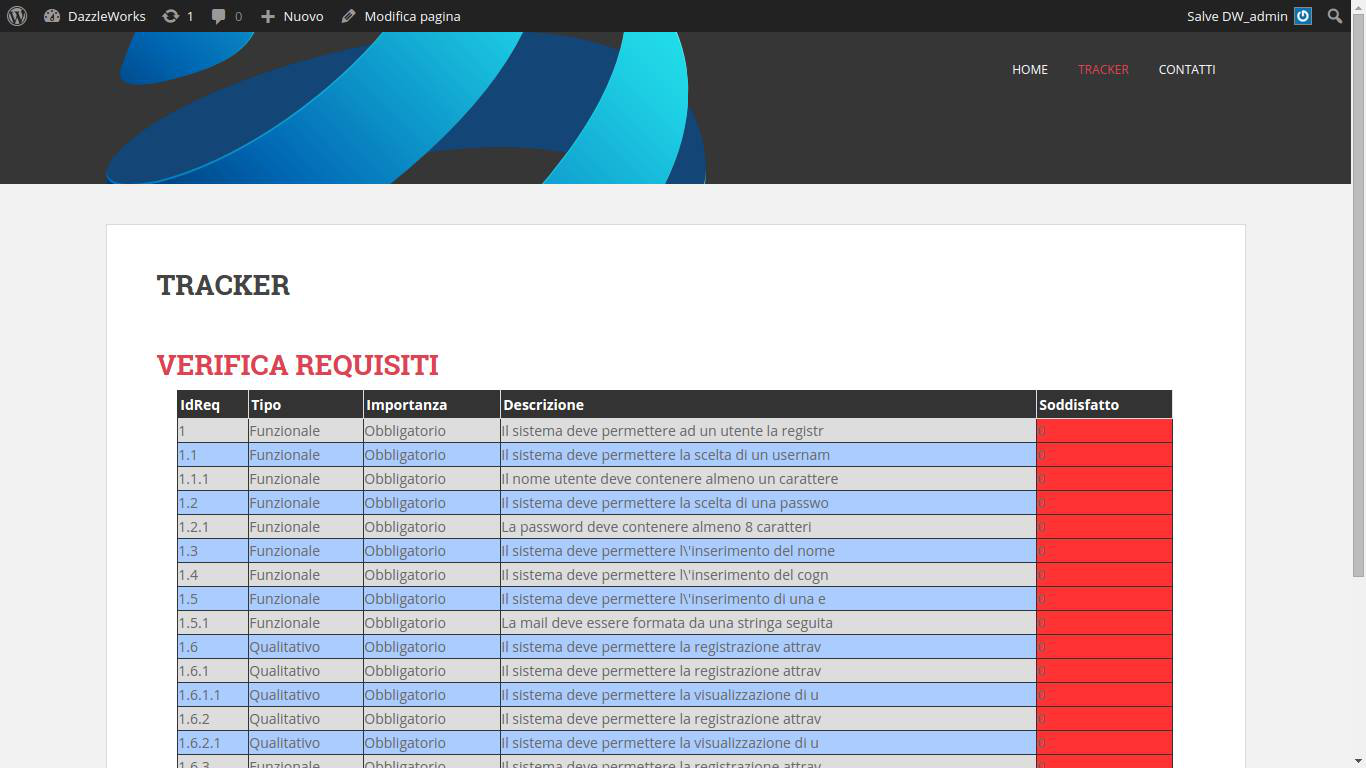
\includegraphics[width=0.7\linewidth]{img/tracker1}
\caption[Pagina riepilogo requisiti]{Pagina riepilogo requisiti}
\label{fig:tracker1}
\end{figure}
\begin{figure}[h]
\centering
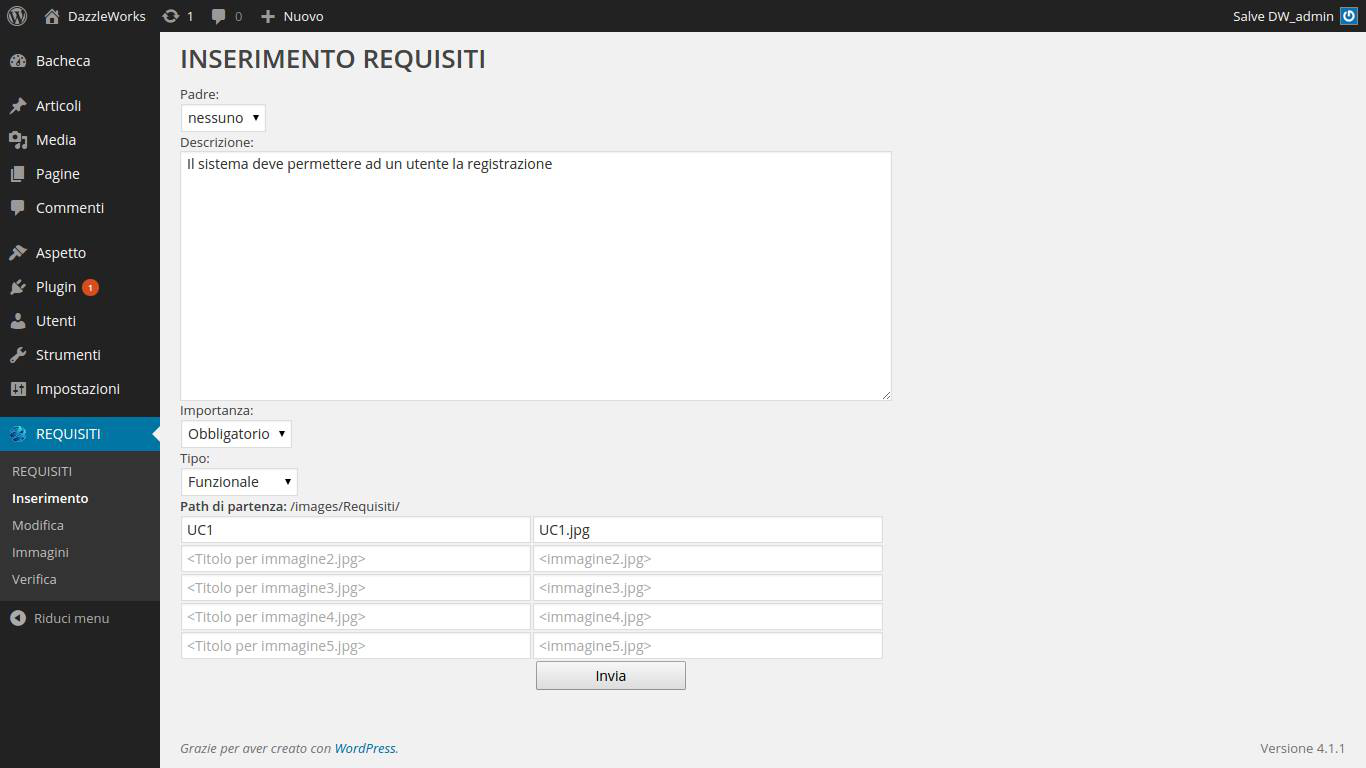
\includegraphics[width=0.7\linewidth]{img/tracker2}
\caption[Pagina inserimento requisito]{Pagina inserimento requisito}
\label{fig:tracker2}
\end{figure}




\newpage
\subsubsection{Progettazione}
Dopo la fase di \textbf{Analisi} si passerà alla fase di \textbf{Progettazione} dove i \textit{Progettisti} dovranno seguire le seguenti regole.\\
\paragraph{Diagrammi UML}
Dovranno essere realizzati i seguenti diagrammi:
\begin{itemize}
	\item Diagrammi delle classi;
	\item Diagrammi dei package;
	\item Diagrammi delle attività;
	\item Diagrammi di sequenza.
\end{itemize}
La lingua utilizzata nella realizzazione dei diagrammi sarà l'\textbf{inglese} e lo standard \gls{UML} sarà 2.0.

\paragraph{Design Pattern}
I \textit{Progettisti} dovranno utilizzare il \gls{design pattern} che ritengono più adatto al contesto per rendere l'applicazione più efficiente possibile. Ogni \gls{design pattern} utilizzato verrà accompagnato da una breve descrizione e da un diagramma che ne esemplifica il funzionamento.

\paragraph{Classi di verifica}
Andranno create delle classi di verifica per testare che tutti i componenti abbiano un comportamento corretto.

\paragraph{Stile di progettazione}
Durante la fase di \textbf{Progettazione} bisognerà fare attenzione a:
\begin{itemize}
	\item \textbf{Ricorsione}: non dovrà essere utilizzata la ricorsione a meno che non sia strettamente necessaria. In quel caso dovrà essere fornita una dimostrazione induttiva sulla correttezza del metodo in questione;
	\item \textbf{Annidamento di cicli}: all'interno di un metodo non dovranno esserci cicli annidati con una profondità maggiore a cinque.
\end{itemize}






\newpage
\subsubsection{Progettazione architetturale}
Lo scopo di questa attività è di fornire un'architettura di alto livello finalizzato ad individuare i sottosistemi che compongono il sistema da realizzare e le loro inter-relazioni di controllo e comunicazione. I compiti principali di questa attività constano nell'individuare le componenti fondamentali e i design pattern che serviranno a comporre lo scheletro dell'architettura. Sarà inoltre necessario individuare le componenti esterne che andranno ad interagire con il software e andranno definite di conseguenze le relative interfacce.
 \begin{itemize}
 	\item \textbf{Identificazione dei componenti: }consiste nell'identificazione dei componenti che il sistema software dovrà avere. I \textit{Progettisti} sono tenuti a studiare le migliore strategie implementative, al fine di soddisfarli, e individuare i design pattern più adatti;
 	\item \textbf{Identificazione delle interfacce: }consiste nell'identificazione delle interfacce necessarie per la comunicazione con le entità esterne. I \textit{Progettisti} sono tenuti a studiare i possibili componenti esterni;
 	\item \textbf{Documentazione dei documenti: }nel momento dell'individuazione di un componente, è necessario procedere alla stesura della sua documentazione. Ogni package avrà le seguenti caratteristiche:
	 	\begin{itemize}
	 		\item \textbf{Identificativo: }ogni package va tracciato con un nome esaustivo con la prima lettera maiuscola. Di seguito si riporta un esempio con package e sotto-package:
	 		{\centering \textbf{Package::SottoPackage1::SottoPackage2 ...};}
	 		\item \textbf{Diagramma: }ogni package deve essere corredato da un diagramma di package in linguaggio UML;
	 		\item \textbf{Descrizione: }ogni package deve avere una descrizione esauriente;
	 		\item \textbf{Sotto-Package: }ogni package deve essere corredato dalla lista di sotto-package che eventualmente contiene;
	 		\item \textbf{Classi contenute: }ogni package deve essere corredato dalla lista delle classi che eventualmente contiene.
	 	\end{itemize}
	 \item \textbf{Tracciamento dei componenti: }ogni requisito deve essere tracciato al componente che lo soddisfa. Per questo i \textit{Progettisti} sono tenuti a utilizzare l'applicativo \textbf{Tracker} per le varie operazioni di tracciamento.
 \end{itemize}
 
\subsubsection{Progettazione architetturale di dettaglio}
Lo scopo di questa attività è fornire un'architettura sufficientemente dettagliata per permettere la codifica e la stesura dei relativi test di unità. I compiti principali di questa attività constano nell'individuare i metodi delle classi definite durante la progettazione ad alto livello, nella documentazione e nella stesura dei test di unità.
	\begin{itemize}
		\item \textbf{Documentazione delle classi: }ogni classe deve avere le seguenti informazioni:
			\begin{itemize}
				\item \textbf{Diagramma: }diagramma UML che rappresenta la classe;
				\item \textbf{Descrizione: }ogni classe deve avere una descrizione esauriente;
				\item \textbf{Attributi: }devono essere indicati li attributi della classe con una breve descrizione;
				\item \textbf{Metodi: }devono essere indicati i metodi della classe con una breve descrizione.
			\end{itemize}
		\item \textbf{Definizione test di unità: } i progettisti dovranno provvedere alla creazione di test di unità per verificare il corretto funzionamento di parti di programma permettendo cosi una precoce individuazione dei bug. I test di unità accurati possono dare una prova certa se un pezzo di codice funziona correttamente, con importanti vantaggi:
			\begin{itemize}
				\item Semplifica le modifiche;
				\item Semplifica l'integrazione;
				\item Supporta la documentazione.
			\end{itemize}
	\end{itemize}

\subsection{Codifica e Convenzioni}
\subsubsection{Linguaggi di codifica}
Dopo un'analisi del capitolato d'appalto e dei requisiti si è deciso che per lo sviluppo del software richiesto si utilizzeranno i linguaggi \gls{HTML5} , \gls{PHP} e \gls{Javascript}.

\subsubsection{Framework e librerie}
Per semplificare la realizzazione della nostra applicazione web si è deciso di utilizzare il \gls{framework} \gls{Angular}, per migliorare le interfacce utente, e la libreria \gls{Chart.js}, utilizzata per generare grafici.

\subsubsection{Convenzioni di codifica}
Di seguito è riportato l'insieme di norme e convenzioni che il gruppo dovrà seguire nella scrittura e documentazione del codice.
L'unica lingua ammessa per i nomi di variabili, metodi e commenti è l'inglese.

\subsubsection{File HTML}

Ogni file \gls{HTML} deve iniziare con il tag <!DOCTYPE html> che serve ad indicare che verrà utilizzata la versione \gls{HTML5}.
Ogni tag deve contenere un id e può contenere una o più classi.
Gli id e le classi dovranno essere contenute in un file .css a parte per mantenere il più possibile la separazione tra \gls{layout} e contenuto.
Le pagine \gls{HTML} devono rispettare gli standard del \gls{W3C}.

\subsubsection{Nomenclatura}
Per l'assegnazione di nomi a variabili, metodi e costanti andranno seguite le seguenti regole:
\begin{itemize}
	\item \textbf{Funzioni:} va utilizzata la notazione mixed case, con la prima lettera minuscola;
	\item \textbf{Variabili:} va utilizzata la notazione mixed case, con la prima lettera minuscola;
	\item \textbf{Costanti:} va scritto il nome interamente in maiuscolo, separando le varie parole con il carattere "\_" (underscore).
\end{itemize}

\subsubsection{Intestazione di un file Javascript}

\begin{flushleft}

/*\\
\vspace{3mm}
\begin{tabular}{l}
	File\\
	Autore\\
	Data\\
	Descrizione\\
\end{tabular}\\
\vspace{5mm}
 Modifiche:\\
 \vspace{3mm}
\begin{tabular}{| c c c c c c c c c |}
	\hline
	Versione & - & Data & - & Programmatore & - & Modifica & - & Descrizione\\
	\hline
	x.y.z & - & aaaa-mm-gg & - & Nome Cognome & - & Funzione & - & Descrizione modifica\\
	\hline
\end{tabular}\\
\vspace{3mm}
*/\\

\end{flushleft}

\begin{itemize}
	\item \textbf{File:} nome del file;
	\item \textbf{Autore:} nome e cognome del creatore del file;
	\item \textbf{Data:} data di creazione del file nel formato aaaa-mm-gg;
	\item \textbf{Descrizione:} poche righe di descrizione delle funzionalità contenute nel file;
	\item \textbf{Cambiamenti:} tabella dello stato di avanzamento del file, contenente tutte le modifiche effettuate :
		\begin{itemize}
			\item \textbf{Versione:} versione una volta effettuata la modifica;
			\item \textbf{Data:} data della modifica;
			\item \textbf{Programmatore:} nome e cognome del programmatore che ha effettuato la modifica;
			\item \textbf{Modifica:} segnatura della funzione a cui è stata apportata una modifica;
			\item \textbf{Descrizione:} breve descrizione della modifica effettuata.
		\end{itemize}
\end{itemize}

\subsubsection{Commenti}

Prima di ogni funzione dovrà essere presente un commento con la seguente forma:

\begin{flushleft}
/*\\
\vspace{3mm}
\begin{tabular}{l}
	Descrizione della funzione\\
	Descrizione dei parametri\\		
	Descrizione del tipo di ritorno\\
\end{tabular}\\
\vspace{3mm}
*/

\end{flushleft}

Ogni variabile di particolare importanza dovrà essere fornita di commento che ne spieghi scopo e funzionamento.






\newpage
\section{Processi di supporto}
\subsection{Processo di documentazione}

	\section{Documenti}
In questo capitolo si descrivono i vari standard adottati da \GRUPPO nella stesura, verifica e approvazione della documentazione da produrre.
\subsection{Template}
Per semplificare la redazione dei documenti è stato creato un template \LaTeX contenente tutte le impostazioni per l'aspetto grafico. \\
Ogni documento dovrà essere realizzato con il template \LaTeX presente nel \gls{repository}. Inoltre è stata scritta una piccola una piccola guida su come usare al meglio il template.
\subsection{Versionamento}
Per ogni documento è obbligatorio specificare la versione. Un numero di versione deve essere nella seguente forma:
\begin{center}
	\emph{X.Y.Z}
\end{center}
dove X, Y, Z sono interi non negativi e non devono contenere zeri iniziali. X è la versione \textit{Major}, Y è la versione \textit{Minor}, e Z e la versione \textit{Patch}.
\begin{itemize}
	\item X: la versione Major (X.y.z | X > 0) identifica la versione di rilascio. Deve essere incrementata se è stata introdotta qualsiasi modifica non retrocompatibile. Le versioni Patch e Minor devono essere reimpostate a 0 quando la versione Major è incrementata. 
	\item Y: la versione Minor (x.Y.z | x > 0) deve essere incrementata se è stata introdotta una nuova funzionalità. La versione Patch deve essere reimpostata a 0 quando la versione Minor è incrementata.
	\item Z: la versione Patch (x.y.Z | x > 0) deve essere incrementata solo se sono state introdotte correzioni retrocompatibili di bug. Una correzione di un bug è definita come una modifica interna che corregge un comportamento errato.
\end{itemize}
Una volta che un pacchetto versionato è stato rilasciato, i contenuti di quella versione \textbf{non devono} essere modificati. Qualsiasi modifica \textbf{deve} essere rilasciata come una nuova versione.

\subsection{Struttura dei documenti}
\subsubsection{Prima pagina}
Ogni documento deve avere in prima pagina le seguenti informazioni:
\begin{itemize}
	\item Nome del progetto;
	\item Logo del gruppo;
	\item Nome del gruppo;
	\item Nome del documento;
	\item La versione del documento;
	\item Cognome e nome dei redattori del documento;
	\item Cognome e nome dei verificatori del documento;
	\item Cognome e nome di chi ha approvato il documento;
	\item Tipo d'uso del documento;
	\item Lista di distribuzione del documento;
	\item Breve descrizione del documento.
\end{itemize}
\subsubsection{Diario delle modifiche}
Nella seconda pagina di ogni documento deve essere presente il diario delle modifiche.\\
Ogni riga del diario delle modifiche contiene:
\begin{itemize}
	\item Una breve descrizione sulle modifiche effettuate;
	\item Cognome e nome di chi ha effettuato la modifica;
	\item Data della modifica;
	\item Versione del documento dopo la modifica.
\end{itemize}

\subsubsection{Indice}
In ogni documento deve essere presente un indice delle sezioni.\\
Nel caso in cui il documento contenga immagini e/o tabelle devono essere presenti anche i relativi indici.

\subsubsection{Formattazione delle pagine}
L'intestazione di ogni pagina contiene:
\begin{itemize}
	\item Logo del gruppo;
	\item La sezione corrente all'interno del documento.
\end{itemize}
A piè di ogni pagina è presente:
\begin{itemize}
	\item Nome e versione del documento;
	\item Pagina corrente nel formato N di T, dove N è il numero della pagina corrente e T è il numero di pagine totali del documento.
\end{itemize}

\subsection{Classificazione documenti}
\subsubsection{Documenti informali}
Si definiscono documenti informali tutti i documenti in fase di sviluppo e devono ancora essere approvati dal \textit{Responsabile di Progetto}. I documenti sono da considerarsi esclusivamente per uso interno e non potranno essere divulgati prima di essere stati verificati ed approvati. 
\subsubsection{Documenti formali}
Si definiscono documenti formali tutti i documenti che sono stati approvati dal \textit{Responsabile di Progetto} e quindi sono pronti ad essere diffusi a terze parti.\\
I documenti pronti per il rilascio dovranno essere rinominati osservando le seguenti regole:
\begin{itemize}
	\item La prima lettera di ogni parola, che non sia una preposizione, deve essere maiuscola;
	\item Gli spazi devono essere sostituiti con il carattere "\_"(underscore);
	\item Tutte le parole devono essere prive di accenti;
	\item La versione del documento verrà aggiunta dopo il nome, e sarà preceduta dal carattere "-"(trattino) e da una "v".
\end{itemize}

\subsection{Norme tipografiche}
Questa sezione racchiude tutte le informazioni riguardanti l'ortografia, la tipografia e l'assunzione di uno stile uniforme in tutti i documenti allo scopo di evitare incoerenze tra le diverse parti del documento.

\subsubsection{Punteggiatura}
\begin{itemize}
	\item Punteggiatura: qualsiasi carattere di punteggiatura non può seguire un carattere di spazio;
	\item Lettere maiuscole: l'uso delle maiuscole è obbligatorio in una serie di casi:
	\begin{itemize}
		\item All'inizio di testo o di una sua parte (capitolo, paragrafo, ecc.);
		\item Dopo il punto, il punto esclamativo, il punto interrogativo;
		\item All'inizio di ogni elemento di un elenco puntato;
		\item Per i ruoli, di progetto, i nomi dei documenti, le fasi di progetto, revisioni di progetto oltre che dove previsto dalla lingua italiana.
	\end{itemize}
	\item Parentesi: il testo racchiuso dentro le parentesi non deve mai iniziare per un carattere di spazio e non deve mai terminare con un carattere di spazio o punteggiatura.
\end{itemize}	

\subsubsection{Stile del testo}
\begin{itemize}
	\item Maiuscolo: l'uso delle maiuscolo è limitato alla trascrizione dei acronimi;
	\item Grassetto: l'uso del grassetto deve essere utilizzato nei seguenti casi: 
	\begin{itemize}
		\item Elenchi puntati: per evidenziare l'oggetto trattato;
		\item Altri casi: è possibile utilizzare il grassetto per evidenziare parole chiave.
	\end{itemize}
	\item Corsivo: l'uso del corsivo deve essere utilizzato nei seguenti casi:
	\begin{itemize}
		\item Citazioni: ogni citazione deve essere scritta in corsivo; 
		\item Documenti: ogni riferimento ad un documento deve essere scritto in corsivo (esempio: \textit{Glossario});
		\item Ruoli: ogni riferimento a figure particolari deve essere scritto in corsivo (esempio: \textit{Verificatore});
		\item Altri casi: è possibile utilizzare il corsivo per evidenziare parole particolarmente significative.
	\end{itemize}
	\item \LaTeX: ogni riferimento a \LaTeX va scritto tramite il comando \verb|\LaTex|.
\end{itemize}

\subsubsection{Composizione del testo}
\begin{itemize}
	\item Elenchi puntati: per redigere un elenco si qualificano gli elementi e si introducono mediante
	i due punti. Dopo i due punti devi andare a capo. Ogni elemento dell'elenco termina con un punto e virgola, eccetto l'ultimo che termina con un punto semplice;
	\item Pedice "G": il pedice "G" viene utilizzato in presenza di termini presenti nel \textit{Glossario};
	\item Note a piè di pagina: ogni nota deve iniziare con la lettera della prima parole maiuscola e non deve essere preceduta dal alcun carattere di spazio. Ogni nota deve terminare con un punto.
\end{itemize}

\subsubsection{Formati ricorrenti}
\begin{itemize}
	\item Nomi propri: l'utilizzo dei nomi propri deve seguire la seguente forma "Cognome Nome";
	\item Percorsi: per gli indirizzi email e gli indirizzi web deve essere usato esclusivamente il comando \LaTeX  \verb|\url|;
	\item Date:  ogni data deve seguire lo standard internazionale per date ed orari ISO 8601:
	\begin{center}
		AAAA.MM.GG
	\end{center}
	dove:
	\begin{itemize}
		\item AAAA: rappresenta il formato dell'anno scritto con quattro cifre;
		\item MM: rappresenta il formato del mese scritto con due cifre;
		\item GG: rappresenta il formato del giorno scritto con due cifre.
	\end{itemize}
	\item Riferimenti ai documenti: ci si riferirà ai vari documenti scrivendo in corsivo il nome del documento e mettendo una lettera maiuscolo per ogni parola che non sia un articolo. Nel caso in cui ci si deve riferire ad una versione specifica del documento, essa andrà indicata alla fine  del nome del documento (esempio: \textit{Norme di Progetto v1.0.0});
	\item Nome del gruppo: ci si riferirà al gruppo solo come "\textit{DazzleWorks}" con il nome del gruppo in corsivo. Per una scrittura corretta del nome è stato creato il comando \LaTeX apposito \verb|\GRUPPO|;
	\item Nome del progetto: ci si riferirà al nome del progetto solo come "\textbf{PREMI}". Per una scrittura corretta del nome è stato creato il comando \LaTeX \verb|\PROGETTO|.
\end{itemize}

\subsubsection{Sigle}
Le sigle potranno essere utilizzate esclusivamente all'interno delle tabelle e diagrammi. Sono presenti le seguente sigle: 
\begin{itemize}
	\item Documenti:
	\begin{itemize}
		\item NdP = \textit{Norme di Progetto};
		\item AdR = \textit{Analisi dei Requisiti};
		\item PdP = \textit{Piano di Progetto};
		\item PdQ = \textit{Piano di Qualifica};
		\item SdF = \textit{Studio di Fattibilità}.
	\end{itemize}
	\item Revisioni:
	\begin{itemize}
		\item RR = \textit{Revisione dei Requisiti};
		\item RP = \textit{Revisione di Progettazione};
		\item RQ = \textit{Revisione di Qualifica};
		\item RA = \textit{Revisione di Accettazione}.
	\end{itemize}
\end{itemize}

\subsection{Componenti grafiche}
\subsubsection{Immagini}
Tutte le immagini dovranno avere il formato \gls{PDF}. In modo da garantire una maggiore qualità dell'immagine in caso di ridimensionamento è consigliato usare il formato \gls{PDF} vettoriale. La conversione di un immagine in formato \gls{PDF} è possibile attraverso il software GIMP\footnote{GNU Image Manipulation Program è un programma per la creazione e modifica di immagini digitali.}, il quale è stato già usato da tutti  i componenti del gruppo. \\ Le immagini devono essere accompagnate da una didascalia che inizia con la parola "Figura" con la prima lettera maiuscola, seguita dal numero della figura, dal carattere "due punti" e da una breve descrizione della figura.
\subsubsection{Tabelle}
Ogni tabella deve essere accompagnata da una didascalia che inizia con la parola "Tabella" con la prima lettera maiuscola, seguita dal numero della tabella, dal carattere "due punti" e da una breve descrizione non banale della tabella.

\subsection{Procedure di avanzamento di un documento}
Quando il redattore ritiene di aver finito la stesura di un documento si devono seguire questi passi esattamente in quest'ordine:
\begin{enumerate}
	\item Il redattore ha il compito di contattare il \textit{Responsabile di Progetto} per informarlo della terminazione della stesura del documento;
	\item Il \textit{Responsabile di Progetto} provvederà a contattare ed assegnare la verifica del documento ad un verificatore disponibile, che non sia in conflitto di interessi;
	\item Il \textit{Verificatore} provvederà alla  verifica del documento;
	\item Nel caso in cui vengano trovati errori nel documento, il \textit{Verificatore} provvederà alla creazione di un ticket di correzione e lo assegnerà al redattore, il quale correggerà gli errori trovati e infine si tornerà di nuovo al passo uno;
	\item Se non sono stati trovati errori, il documento verrà approvato dal \textit{Responsabile di Progetto}. 
\end{enumerate}

	
\newpage
\subsection{Processo di verifica}

	La verifica dei processi, documenti e prodotti è un'attività da eseguire continuamente durante lo sviluppo del progetto. Di conseguenza, servono modalità operative chiare e dettagliate per i \textit{Verificatori}, in modo da uniformare le attività di verifica svolte ed ottenere il miglior risultato possibile. Si descrivono ora le modalità ordinate e puntuali di verifica di processi, documenti, attività e codice alle quali ci si riferirà in questo documento e alle quali i \textit{Verificatori} dovranno attenersi.

\subsubsection{Tecniche di analisi}

	\paragraph{Analisi statica}
		\subparagraph{Walkthrough:}
Cosiddetta lettura a pettine, questa tecnica di analisi prevede una lettura critica del codice o del documento prodotto. Tale tecnica è molto dispendiosa in termini di risorse, poiché viene applicata all'intero documento, senza avere una precisa idea di quale sia il tipo di anomalia e di dove ricercarla. Essa è però necessaria nelle prime fasi del progetto, vista l'inesperienza da parte del gruppo nell'attuare un tipo di verifica più precisa e mirata. Dopo una prima fase di lettura ed identificazione degli errori, si procede alla discussione degli stessi, proponendo le modifiche da apportare per garantirne la correzione. Il passo finale consiste nell'applicare le modifiche proposte, redigendo un rapporto preciso che elenchi le modifiche effettuate. Una caratteristica di questo tipo di analisi è che richiede l'utilizzo di più risorse umane;
	\subparagraph{Inspection:}
Cosiddetta ricerca selettiva, questa tecnica di analisi presuppone l'esperienza da parte del verificatore nell'individuare gli errori e le anomalie più frequenti. A tal scopo è necessaria una lista di controllo stilata in una precedente analisi di tipo \gls{walkthrough} nella quale sono elencate le sezioni critiche. Questo ci consente una verifica più rapida e meno risorse umane. Dopo aver terminato l'analisi, è necessario stilare un rapporto di verifica.

	\paragraph{Analisi dinamica}
Si applica solo alle componenti software e consiste nella verifica e validazione attraverso i test. Per garantire la correttezza è necessario che i test siano ripetibili: dato lo stesso input il test deve produrre sempre lo stesso output. Solo i test con queste caratteristiche riescono a verificare la correttezza del prodotto.\\
Per ogni test deve essere definito:
\begin{itemize}
	\item \textbf{Ambiente: }consiste nel sistema hardware e software sul quale andrà eseguito il test;
	\item \textbf{Specifica dei valori: }consiste nel definire i valori di input e i valori attesi per i parametri di output;
	\item \textbf{Procedura: }consiste nel definire il modo in cui i test dovranno essere effettuati, specificando un eventuale ordine e come dovranno essere interpretati i risultati.  
\end{itemize}

	\paragraph{Test}
		\subparagraph{Test di unità:}
		Il test di unità verifica che ogni singola unità funzioni correttamente. In particolare si verifica che i requisiti per quella determinata unità siano soddisfatti.
		\subparagraph{Test di integrazione:}
		Il test di integrazione rappresenta l'estensione logica del test di unità. Consiste nella combinazione di due unità già sottoposte a test in un solo componente e nel test dell'interfaccia presente tra le due. Il test di integrazione consente di individuare i problemi che si verificano quando due unità si combinano. Per effettuare tali test si farà uso di classi appositamente create per simulare e verificare l'interazione.
		\subparagraph{Test di sistema:}
		Il test di sistema consiste nella validazione del sistema. Viene eseguito quando si ritiene che il prodotto sia giunto ad una versione definitiva, verificando la completa copertura dei requisiti da parte del prodotto.
		\subparagraph{Test di regressione:}
		Il test di regressione va eseguito ogni volta che viene modificata un'implementazione in un programma. A tale scopo, è possibile eseguire nuovamente i test esistenti sul codice modificato per stabilire se le modifiche apportate hanno alterato elementi precedentemente funzionanti. Se necessario è anche possibile scrivere nuovi test.
		\subparagraph{Test di accettazione:}
		Il test di accettazione consiste nel collaudo del sistema eseguito dal committente. Se l'esito è positivo si può procedere al rilascio ufficiale del prodotto.

\subsubsection{Verifica dei documenti}
La verifica dei documenti verrà eseguita ogni volta che sarà effettuata una modifica ad un documento e debba essere approvato.
Per una corretta verifica di un documento vanno seguite le seguenti pratiche:

\begin{itemize}
	\item \textbf{Controllo tipografico: }tramite l'utilizzo di TeXstudio verranno individuati errori tipografici presenti nel documento;
	\item \textbf{Controllo lessicale: }il \textit{Verificatore} dovrà controllare che il documento non presenti errori lessicali attraverso un'attenta analisi del testo utilizzando la tecnica \gls{inspection} o \gls{walkthrough};
	\item \textbf{Controllo glossario: }il \textit{Verificatore} dovrà controllare che ogni parola, nel testo, presente nel glossario sia correttamente evidenziata;
	\item \textbf{Controllo contenuto: }il \textit{Verificatore} dovrà controllare che il documento contenga tutto il necessario e che sia impaginato adeguatamente;
	\item \textbf{Rispetto delle norme del progetto: }il \textit{Verificatore} dovrà controllare che il documento segua le norme di progetto stabilite;
	\item \textbf{Lista di controllo: }si dovrà stilare una lista di errori più frequenti, per semplificare le successive verifiche dei documenti;
	\item \textbf{Rispetto \gls{indice Gulpease}: }il \textit{Verificatore} dovrà calcolare e controllare, per ogni documento, che gli \gls{indici di Gulpease} ricadano nel range di valori specificato nel \textit{Piano di Qualifica}, altrimenti si dovrà effettuare una ricerca \gls{walkthrough} delle frasi troppo lunghe e complesse;
	\item \textbf{Segnalazione errori: }una volta completata la verifica di un documento, se sono stati riscontrati errori, il \textit{Verificatore} dovrà aprire dei \gls{ticket} per segnalarli.
\end{itemize}
	
\subsubsection{Verifica dei diagrammi}
I diagrammi devono essere verificati manualmente dal \textit{Verificatore} che deve controllare che aderiscano correttamente allo standard \gls{UML} 2.0.
In particolare deve controllare che i diagrammi di flusso siano rappresentati in maniera corretta e che i \gls{casi d'uso} utilizzino correttamente le inclusioni e le estensioni.


\newpage
\section{Processi organizzativi}
\subsection{Processo di gestione del progetto}
	La responsabilità di gestione del progetto è attribuita al \textit{Responsabile di Progetto}. \\
Utilizzando tutti gli strumenti a disposizione il \textit{Responsabile di Progetto} avrà il compito di:
\begin{itemize}
	\item Pianificare le attività;
	\item Gestire le risorse;
	\item Analizzare e prevenire i rischi.
\end{itemize}

\subsubsection{Pianificazione delle attività}
Per pianificare le varie attività da svolgere il \textit{Responsabile di Progetto} dovrà utilizzare \gls{GanttProject} per realizzare i diagrammi di \gls{Gantt}.

\subsubsection{Coordinazione e gestione delle risorse}
Per gestire le risorse durante lo sviluppo del progetto, il \textit{Responsabile di Progetto} dovrà pianificare la quantità di ore che ogni risorsa dovrà dedicare a ciascuna attività.\\
Si è deciso di utilizzare il servizio di gestione dei \gls{task} e creazione di \gls{milestone} offerto da \gls{GitHub} spiegato nella sezione \ref{repository}. Questo permette di accentrare le informazioni in un solo ambiente.

\subsubsection{Analisi e prevenzione dei rischi}
Durante l'avanzamento del progetto, il \textit{Responsabile di Progetto} deve monitorare costantemente il verificarsi dei rischi descritti nel \textit{Piano di Progetto v2.0.0}. La valutazione dei rischi deve essere aggiornata al mutare delle situazioni di pericolo, in occasione di significative modifiche al processo produttivo oppure all'introduzione di nuove tecnologie. Una volta completata la valutazione dei rischi si dovrà redigere una relazione scritta, modificando e aggiornando il \textit{Piano di Progetto}, contenente le misure di prevenzione previste e il loro programma di attuazione.





\newpage
\appendix
\section{Lista di controllo}
Di seguito verrà presentata la lista degli errori più comuni trovati durante le verifiche dei documenti:
\begin{itemize}
	\item \textbf{Norme stilistiche:} la conoscenza \textbf{non} approfondita delle norme per la stesura dei documenti potrebbe portare a errori:
		\begin{itemize}
			\item Nel caso degli elenchi potrebbero esserci elementi che non iniziano con la lettera maiuscola;
			\item Nel caso degli elenchi potrebbe non terminare con il "." nel caso dell'ultimo elemento oppure potrebbe mancare il ";" per uno o più elementi tranne l'ultimo; 
			\item Potrebbe mancare la marcatura "G" in pedice per i termini presenti nel \textit{Glossario};
			\item Il non utilizzo del grassetto per le fasi principali del progetto, il corsivo per i documenti e i ruoli di progetto;
			\item Le note a piè di pagina che non iniziano con una maiuscola e non finiscono con il ".".
		\end{itemize}
	\item \textbf{Lingua italiana:} 
		\begin{itemize}
			\item Più tempi verbali all'interno della stessa frase;
			\item Utilizzo di termini con significato ambiguo.
		\end{itemize}
	\item \textbf{\LaTeX:} non viene considerato il carattere di spaziatura dopo l'inserimento dei  comandi \LaTeX;
	\item \textbf{Altro:} errori dovuti a distrazioni e/o errori di battitura.
\end{itemize}



%\newpage

% ...

%\printglossaries

\end{document}
